\documentclass[10pt]{ctexart}
\CTEXsetup[format={\Large\bfseries}]{section}
\usepackage{cite}
\usepackage{graphicx}
\usepackage{subfigure}
\usepackage{booktabs}
\usepackage{geometry}
\usepackage{float}
\usepackage{amsmath}
\usepackage{lmodern}
\usepackage{multirow}
\usepackage{CJK}
\usepackage[marginal]{footmisc}
\usepackage{enumerate}
\renewcommand{\thefootnote}{}
\usepackage{multicol} % 用于实现在同一页中实现不同的分栏
\geometry{a4paper,scale=0.8}
% \usepackage{cjk}
% \newcommand{\upcite}[1]{\textsuperscript{\textsuperscript{\cite{#1}}}}
\usepackage{authblk}
 

\newcommand{\upcite}[1]{\textsuperscript{\textsuperscript{\cite{#1}}}}
\begin{document}
\setlength{\columnsep}{25pt} 
% \author{王树立}
\date{}
\bibliographystyle{unsrt}
\title{勺型网络:用于landsat遥感图像云检测的新型网络}
\author[]{王树立\thanks{\noindent \textbf{通讯作者}: E-mail:wangshuli18@mails.ucas.ac.cn}\ , 唐海蓉}
\affil[]{\small(中国科学院空天信息创新研究院,北京 100094; 中国科学院大学,北京 100049;\\ 中国科学院空间信息处理与应用系统技术重点实验室,北京 100190)}
\renewcommand\Authands{\, }
\pagestyle{empty} % 没有页眉和页脚
\maketitle
\pagestyle{empty} % 去掉第二页及其后各页的页码
\thispagestyle{empty} % 去掉当前页的页码
% \section*{}
\noindent\textbf{摘\ 要}\ 云检测是遥感图像应用的关键预处理步骤,而基于神经网络的云检测正逐渐成为一个重要的研究方向。本文针对目前神经网络模型存在的细节信息易损失、光谱信息未能充分利用、参数量大、计算复杂等不足,提出了一种新型的、轻量的网络,称为勺型网络(Spoon-Net,简称S-Net),用于Landsat遥感图像的云检测。S-Net分为两个阶段,第一阶段,使用$1*1$的卷积核对遥感图像进行光谱特征提取;第二阶段,使用encoder-decoder框架对遥感图像进行空间特征提取。同时为了防止已提取的光谱特征被破坏,本文引入分组卷积,对第一阶段提取的每一层光谱通道单独进行卷积。模型在Landsat8 Biome数据做训练并估计,在模型参数量只有U-Net的八十分之一(0.34M)的情况下,取得了全面优于U-Net的实验结果,达到了95.34\%的准确率。

\noindent\textbf{关键词}\ Landsat, 云检测,神经网络

\noindent\textbf{中图分类号}:TP751.2

\begin{center}
    \Large
    Spoon network: A new network structure of Landsat imagery cloud detection
    \\[10pt]
    \normalsize 
    Wang Shuli, Tang Hairong, Ji Luyan
    \\[8pt]
    \small
    (Aerospace Information Research Institutue, Chinese Academy of Sciences, Beijing 100094, China;
    
    University of Chinese Academy of Sciences, Beijing 100049, China; Key Laboratory of Technology in Geo-spatial Information Processing and Application System, Beijing 100190, China)
\end{center}

\noindent\textbf{Abstract}\ Cloud detection is the key preprocessing step of remote sensing image application, and cloud detection based on neural network is becoming an important research direction. In this paper, a new and lightweight neural network called spoon net (S-Net for short) is proposed for Landsat remote sensing image cloud detection in view of the shortcomings of the current neural network model, such as the loss of detail information, insufficient use of spectral information, large amount of parameters and complex calculation. S-Net is divided into two stages. In the first stage, we use convolution check of $1 * 1$ to extract spectral features of remote sensing image; in the second stage, we use encoder decoder framework to extract spatial features of remote sensing image. At the same time, in order to prevent the extracted spectral features from being destroyed, this paper introduces the group convolution, and convolutes each layer of spectral channel extracted in the first stage separately. The model is trained and estimated with landsat8 biome data. When the model parameters are only one eightieth of U-Net (0.34M), the experimental results are better than U-Net in all respects, and the accuracy is 95.34\%.

\noindent\textbf{Keywords}\ Landsat, cloud detection, neural network

% \columnseprule=1pt         % 实现插入分隔线
\begin{multicols}{2} 

\setcounter{section}{0} % 从0开始计数
\section*{引言}
以Landsat卫星为代表的遥感数据在当今社会的生产和生活中扮演着至关重要的角色,在农业产量估算\upcite{prasad2006crop}、变化检测\upcite{verbesselt2010detecting}、灾难评估\upcite{joyce2009review}等方面发挥着重要的作用。随着科技的发展,遥感数据变得越来越多,且越来越容易获得。海量的多波段遥感数据也急切需要高效率和高鲁棒性的算法进行处理和数据挖掘。然而,在Landsat数据集上,每年有高达40\%的像素被云覆盖\upcite{ju2008availability},云层作为光学遥感图像的主要污染源,对遥感图像的应用造成了极大的限制。所以对云检测算法的研究一直是遥感领域中的热点。

实时的云检测算法目前可以分为两类:基于光谱信息的和基于空间信息的。
光谱是地物最本质的特征之一,不同的地物有不同的辐射与反射特性,云在反射波段表现为亮目标,发射波段表现为暗目标。基于光谱信息的方法\upcite{sun2018cloud}有些直接利用波段特征,也有些通过非线性映射构造新的特征(如波段比值、波段指数等),并精心设置阈值以更好地区分地物。Irish等人\upcite{irish2006characterization}提出的ACCA使用 Landsat7 ETM +谱段 2- 6 的信息,获得暖云掩码,冷云掩码,非云掩码和雪掩码。Zhu等人提出的FMask算法\upcite{zhu2012object}用到了Landsat几乎所有的波段,通过设置亮度阈值、色度阈值、温度阈值、NDVI、NDSI等,通过决策树选择出两个潜在云掩膜,并组合成最终的结果。此类方法实现简单,便于理解,可解释性强,在一般情况下可以取得较好的效果,但当地面覆盖了冰、雪、沙漠,或云为薄卷云、小积云时,云和地面难以区分。

在空间上,云的表现则更加多样,有小面积的碎云,一大片的层云,有较厚的积云,也有较薄的卷云,但云是由水汽聚集而成,处于中心位置的云更加容易识别,边缘部分或者较为模糊的云可以利用空间分布进行识别。一些方法通过提取图像纹理特征,如LBP特征、HOG特征、haar特征等,利用云与地物在空间上结构的不同进行区分。还有一些文章将高分辨率图像切割成一张张子图或超像素,如SLIC\upcite{achanta2012slic},再利用机器学习的方法对子图或超像素进行分类,如SVM\upcite{lee2004cloud}、MLP\upcite{tian1999study}。这些方法一方面降低了图像的分辨率,另一方面受到云多样性的影响在处理薄云、小面积云时效果并不佳。

近年来,深度学习在自然语言处理、降维、图像分类、目标检测、语义分割等方面取得了诸多成果。从AlexNet开始,深度学习开始席卷图像处理领域。
相较许多传统方法需要人工构造特征和精心选择阈值的特点,深度学习通过构造多层神经网络,自动提取特征和阈值。而且,精心选择的神经网络可以构造出高维特征,更加有效地区分云与地物。

目前有很多方法将全卷积网络应用于遥感图像的云检测。Jeppesena等人\upcite{jeppesen2019cloud}将U-Net应用于Landsat遥感图像云检测。Chai等人\upcite{chai2019cloud}将SegNet应用于Landsat图像。Hughes等人\upcite{hughes2019high}将FCN应用于云检测。这些方法是对已有模型在遥感图像云检测任务上的应用,都取得了不错的效果。

但这些方法存在两个缺点:
1.对地物的光谱特征提取不足。这些模型没有充分利用遥感图像多波段特性和云在光谱上的重要属性,混合提取光谱特征与空间特征(一阶段的),使得光谱特征提取困难并且难以解释,造成了遥感光谱信息的浪费。
2. 过于重视遥感图像的空间特征。这导致小的碎云容易被忽视,边缘细节容易被丢失,分类结果过于平滑,同时也造成了参数量巨大与计算冗余。

为了充分利用云的光谱属性,保持云的边缘细节,本文提出了一个新颖的、简单的、有效的网络,称为勺型网络(Spoon-Net,简称S-Net)用于Landsat图像云检测。网络主要包括两个阶段。
第一阶段,光谱特征提取阶段。在这一阶段,我们完全使用$1*1$的卷积核,不受空间信息干扰,专门对图像进行光谱特征提取。而且$1*1$卷积核可以在不降低图像分辨率的前提下,使得后续的空间特征更加容易被提取。
第二阶段,空间特征提取阶段。这一阶段,采用轻量化的encoder-decoder框架。进一步,我们不会破坏已提取的光谱特征,而是采用组卷积(Group Conv)的方式,将第一部分得到的每一种光谱特征作为一组进行单独的卷积。由于光谱特征提取阶段的存在,组卷积在大大减少参数量的同时,有效提取空间特征。
最终的分类结果将像素分为云与非云两类。实验结果表明,S-Net可以在模型参数大大减小的情况下,明显提高云检测精度。

\section[]{数据与方法}
\subsection{数据}
本文采用的光学遥感卫星数据集来自美国航空航天局(NASA) Landsat8卫星。2013年2月11日, NASA成功发射Landsat-8卫星。Landsat-8卫星上携带两个传感器,分别是OLI陆地成像仪和TIRS热红外传感器。OLI提供9个波段,波段范围从0.43um到2.30um;TIRS提供地表温度数据,包括两个波段,波段范围从10.60um到12.51um,具体信息见表\ref{landsatBand}。Landsat系列卫星每16天可以实现一次全球覆盖。

\begin{table}[H]
    \caption{Landsat8波段信息}
    %英文标题begin
    \addtocounter{table}{-1}
    \vspace{-5pt}
    %\SetEnglishCaption
    \renewcommand{\tablename}{Tab}
    \caption{Landsat8 band information}
    \renewcommand{\tablename}{表}
    \vspace{5pt}
    %英文标题end

    \centering
    \resizebox{\linewidth}{!}{
    \begin{tabular}{ccccc}
    \hline
    传感器类型& 编号&波段 &波长范围($\mu m$)& 空间分辨率(m)\\
    \hline
    \multirow{9}*{OLI}& 1& Coastal& 0.433-0.453& 30\\
    ~&2& Blue& 0.450-0.515& 30\\
    ~&3& Green& 0.525-0.600& 30\\
    ~&4& Red& 0.630-0.680& 30\\
    ~&5& NIR& 0.845-0.885& 30\\
    ~&6& SWIR1& 1.56-1.66& 30\\
    ~&7& SWIR2& 2.1-2.3& 30\\
    ~&8& Pan& 0.5-0.68& 15\\
    ~&9& Cirrus& 1.36-1.39& 30\\
    \hline
    \multirow{2}*{TIRS}& 10& TIRS1& 10.60-11.19& 100\\
    ~& 11& TIRS2& 11.50-12.51& 100\\
    \hline
    \end{tabular}}
    \label{landsatBand}
    \end{table}


为了对模型进行训练与测试,本文利用已有的全球云和云影验证数据集
“L8 Biome Cloud Validation Masks”\upcite{foga2017cloud_data},该数据集共有96景图片,包含8个种类的下垫面。%(including Barren, Forest,Grass/Crops, Shrubland, Snow/Ice, Urban, Water, Wetlands。
% \end{multicols}

% \begin{figure}[H]
%     \centering
%     \includegraphics[scale=0.5]{../pic/BiomeData.png}
%     \caption{Global distribution of the 96 unique Landsat 8 Cloud Cover Assessment (CCA) scenes.}
%     \label{fig:label}
% \end{figure}

% \begin{multicols}{2} 
每景图片的标签均是人工标注,可信度较高。每个文件包含.TIF格式的Landsat 8 Level-1数据文件、质量文件和.img(ENVI)格式的真值标签,人工标志位如表\ref{BiomeFlag}所示。

\begin{table}[H]
    \caption{L8 Biome 数据人工标注标志位}
    %英文标题begin
    \addtocounter{table}{-1}
    \vspace{-5pt}
    %\SetEnglishCaption
    \renewcommand{\tablename}{Tab}
    \caption{flag of Landsat8 biome}
    \renewcommand{\tablename}{表}
    \vspace{5pt}
    %英文标题end

    \centering
    \resizebox{\linewidth}{!}{
    \begin{tabular}{cccccc}
    \hline
    数值& 0& 64& 128& 192& 255\\
    \hline
    解释&	填充值& 云阴影& 非云像素 &薄云& 云\\
    \hline
    \end{tabular}}
    
    \label{BiomeFlag}
    \end{table}

根据云量百分比的多少,‘L8 Biome’中96景分为clear, midcloud, cloud三种,每种各占三分之一,云量低于35\%的为clear,云量高于65\%的为cloud,云量介于35\%与65\%之间的为midcloud。本文使用midcloud的所有数据,共32景做实验,每种地物有4景。我们将数据标签简单地分为云与非云两类,将每景L8图像均匀切割为$256*256$大小的子图,切割时过滤掉带填充值的图片,因此图像边缘的填充像素并不会出现在训练与测试的步骤中。选择除了全色波段的所有波段(TIRS数据的空间分辨率已重采样到30m),共10个波段,训练集与测试集的比例为6:4,训练集有10247张子图,测试集有6932张子图。

\subsection{Encoder-decoder框架与改进}
Encoder-decoder框架是图像分割领域的主流框架。Encoder的作用是提取空间特征,decoder的作用是解析空间特征,并将图像还原到原来的大小以获得像素级别的分类,跳层连接统筹兼顾感受野与空间分辨率。FCN\upcite{FCN}与U-Net\upcite{ronneberger2015unet}均采用这种框架。但该框架一般应用于灰度图像与彩色图像,若应用于遥感图像云检测,虽然可以涉及光谱维度的计算,但主要是在提取空间特征,对光谱特征的提取能力不足。
本文考虑遥感图像多波段的特点,对encoder-decoder框架进行改进,将其扩充为两阶段,分步提取光谱特征与空间特征。

\begin{figure}[H]
    \centering
    \subfigure[encoder-decoder 框架.]{
        \begin{minipage}[b]{0.7\linewidth}
        \resizebox{\linewidth}{!}{
        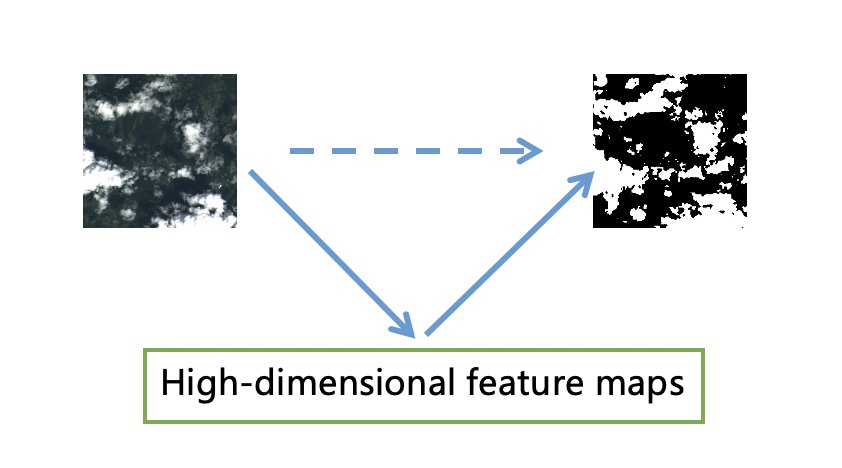
\includegraphics[]{../pic/en-decoder.jpg}}
        \label{fig:encoder-decoder}
        \end{minipage}
        }
    \subfigure[Spoon-Net 框架.]{
        \begin{minipage}[b]{\linewidth}
        \resizebox{\linewidth}{!}{
        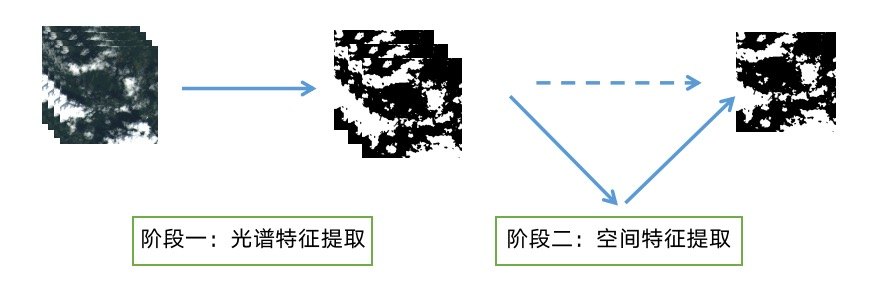
\includegraphics[]{../pic/spoon_simple.jpg}}
        \label{fig:Spoon-net}
        \end{minipage}
        }
    \caption{encoder-decoder框架 与 Spoon-net 对比}
    %英文标题begin
    \addtocounter{figure}{-1}
    \vspace{-5pt}
    %\SetEnglishCaption
    \renewcommand{\figurename}{Fig}
    \caption{Comparison of encoder-decoder framework and Spoon-net}
    \renewcommand{\figurename}{图}
    %英文标题end

    \label{fig:spoon_simple}
\end{figure}

\subsection{网络结构}
本文提出的S-Net是一个两阶段模型,第一阶段是光谱特征提取阶段,第二阶段是空间特征提取阶段。详细模型结构如图\ref{fig_myModel}所示,每个矩形框上面的数字代表特征图的个数。
\end{multicols}

\begin{figure}[H]
    \centering
    \resizebox{\linewidth}{!}{
    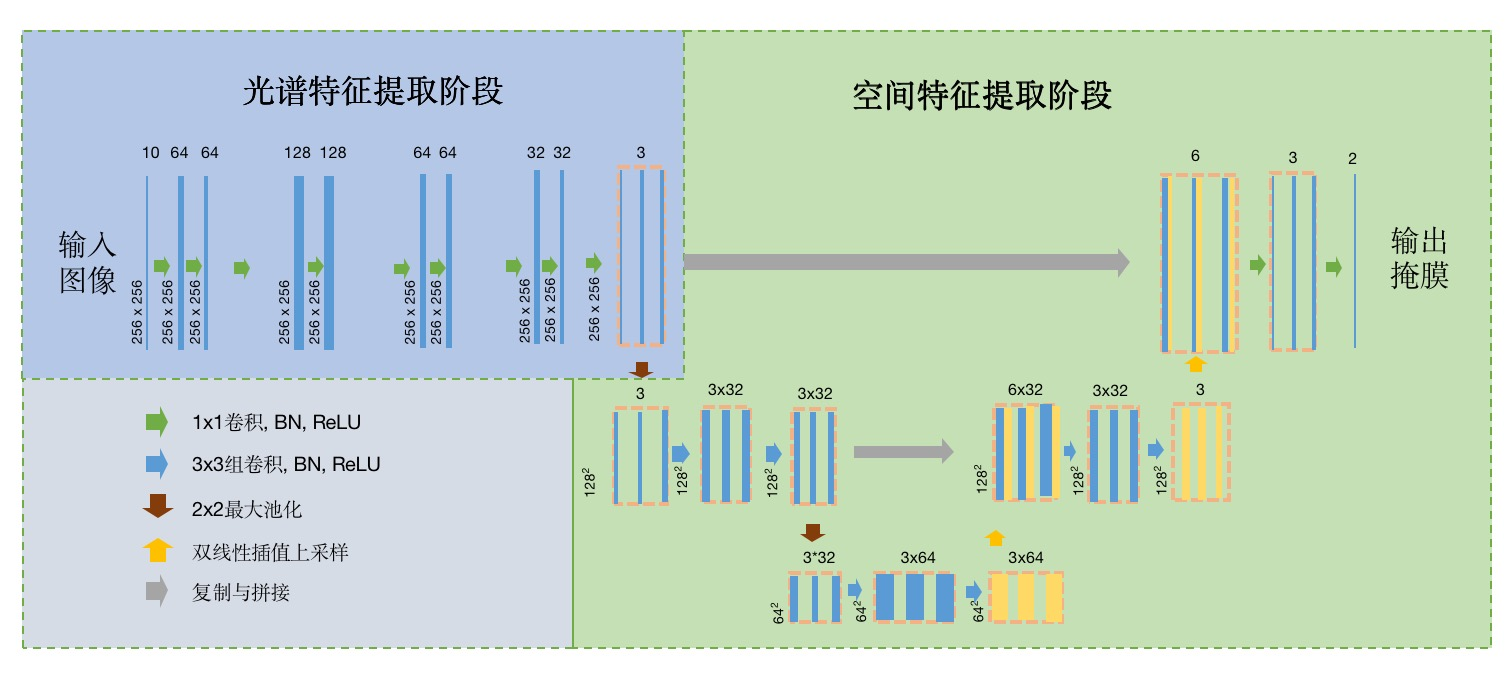
\includegraphics[scale=1]{../pic/spoon.jpg}}
    \caption{Spoon-net 详细结构.}
    %英文标题begin
    \addtocounter{figure}{-1}
    \vspace{-5pt}
    %\SetEnglishCaption
    \renewcommand{\figurename}{Fig}
    \caption{Spoon-net framework}
    \renewcommand{\figurename}{图}
    %英文标题end
    \label{fig_myModel}
\end{figure}
\begin{multicols}{2} 
1. 光谱特征提取阶段。 该阶段使用$1*1$的卷积核对单个像素进行计算,提取出三个最优的光谱特征。因为不涉及到空间信息,所以可以有效保持图像的细节。多层$1*1$的卷积操作等价于一个多层感知机(MLP),MLP可以有效提取非线性光谱特征,为后续分类提供良好的基础,并且不会降低图像分辨率。这一阶段输出的每一层特征图都是一种有效的光谱特征,类似于NDVI、NDWI等,但远比它们复杂得多,更加具有非线性,也更有效。详细结构如图\ref{pic:straight}所示。

\begin{figure}[H]
    \centering
    \resizebox{\linewidth}{!}{
    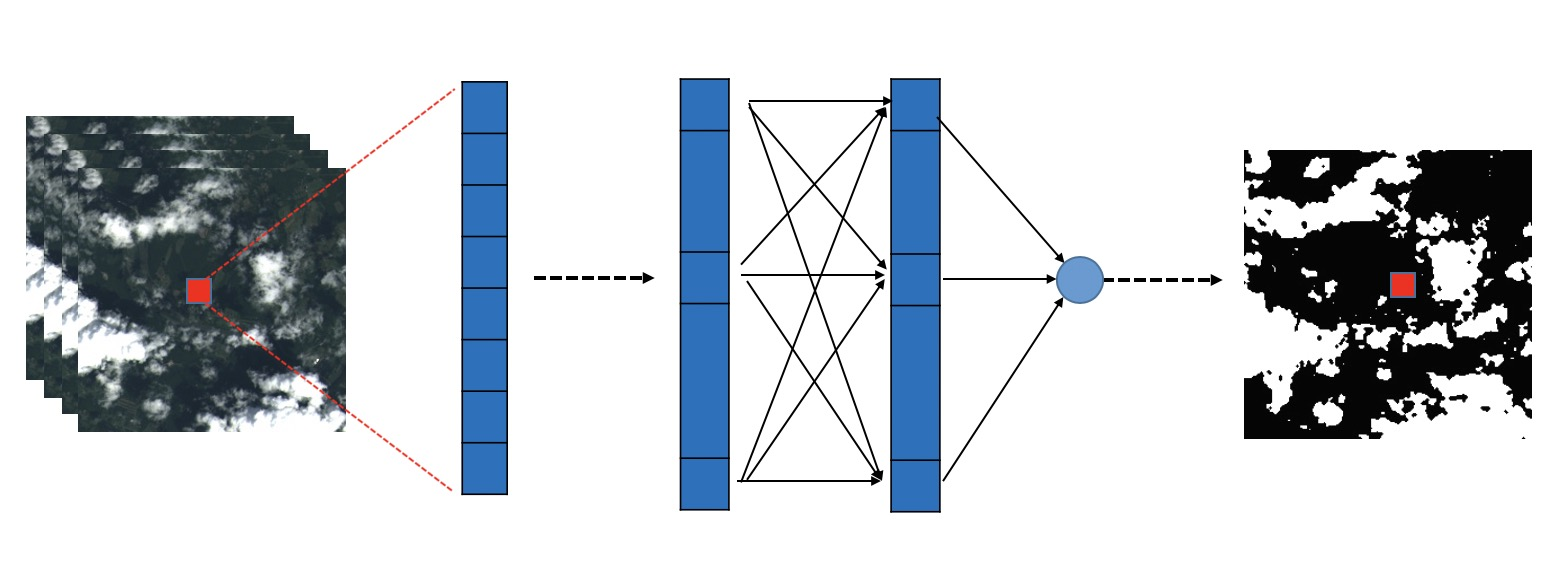
\includegraphics[scale=1]{../pic/part1.jpg}}
    \caption[]{阶段一: 所有的卷积核都是$1*1$大小的,等价于多层感知机。}
    %英文标题begin
    \addtocounter{figure}{-1}
    \vspace{-5pt}
    %\SetEnglishCaption
    \renewcommand{\figurename}{Fig}
    \caption{stage 1: all convolutional kernels are $1*1$, which is equivalent to multi-layer perceptron.}
    \renewcommand{\figurename}{图}
    %英文标题end
    \label{pic:straight}
\end{figure}

这一阶段生成的光谱特征,不仅会用于第二阶段的空间特征提取,还会以跳层连接的方式直接参与最终的分类,并且分类层的卷积核也是$1*1$,这意味着我们的网络有足够的能力保证分割结果的细节。

2. 空间信息提取阶段。在第一阶段提取的光谱特征基础上,通过进一步的区域空间信息与上下文信息的提取,充分利用空间信息,有效减少了云检测的虚警率。同时为了使模型更加轻量化,我们采用浅层神经网络与组卷积。详细的空间特征提取过程如图\ref{pic:part2}所示。
\begin{figure}[H]
    \centering
    \resizebox{\linewidth}{!}{
    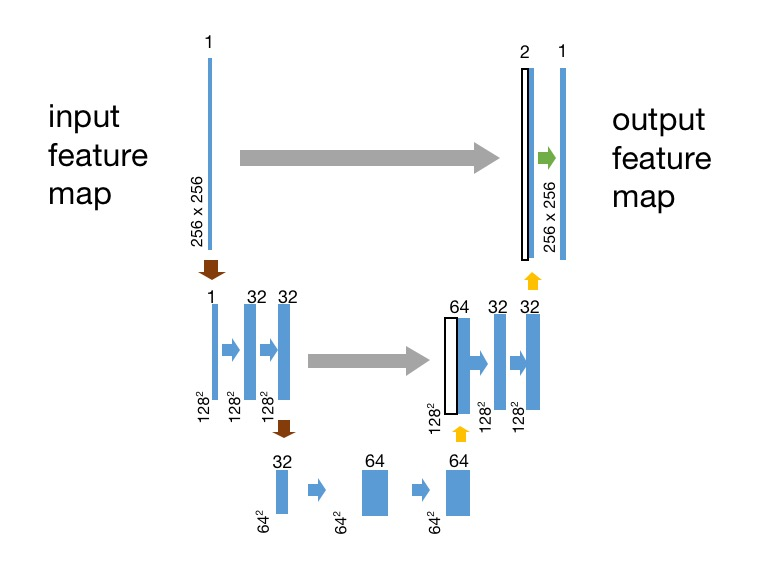
\includegraphics[scale=1]{../pic/groupcov.jpg}}
    \caption[]{阶段二: 每组特征图的卷积过程。}
    %英文标题begin
    \addtocounter{figure}{-1}
    \vspace{-5pt}
    %\SetEnglishCaption
    \renewcommand{\figurename}{Fig}
    \caption{stage 2: Convolution process of each group.}
    \renewcommand{\figurename}{图}
    %英文标题end
    \label{pic:part2}
\end{figure}

空间特征提取采用浅层(2层)的encoder-decoder结构,除了最后的分类层是$1*1$的卷积核,其余卷积核为$3*3$;利用最大池化层降低图像分辨率,扩大感受野;将高分辨率的特征图通过跳层连接与低分辨率的特征图进行拼接,以检测不同大小的目标。

同时,本文引入组卷积的概念,避免在光谱上的重复计算,更加有效提取空间信息。图\ref{pic:GC}展示了组卷积与普通卷积的区别。普通卷积会使所有的特征图参与计算,而组卷积将特征图与卷积核分组,每组卷积核只会与该组内的特征图进行卷积。在本文中,组卷积具有明确的意义,将第一阶段提取的每种特征作为单独的一组,针对性地提取空间信息,也意味着这一阶段不会重复提取或破坏已有的光谱特征,专注于空间特征的提取。

\begin{figure}[H]
    \centering
    \subfigure[普通卷积,$c_o$个卷积核.]{
        \begin{minipage}[b]{\linewidth}
        \resizebox{\linewidth}{!}{
        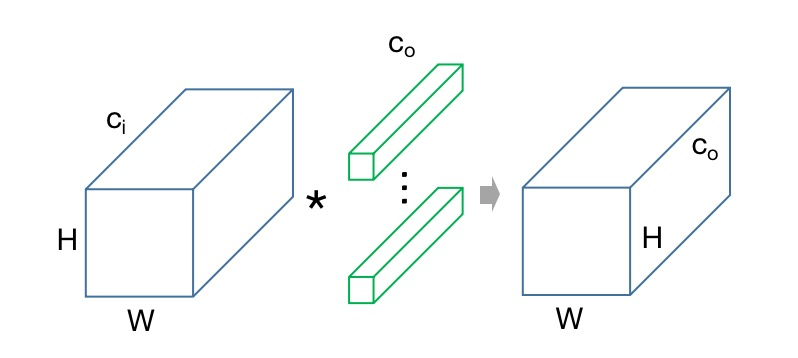
\includegraphics[]{../pic/conv.jpg}}
        \label{fig:encoder-decoder}
        \end{minipage}
        }
    \subfigure[组卷积,$c_o$个卷积核分为2组.]{
        \begin{minipage}[b]{\linewidth}
        \resizebox{\linewidth}{!}{
        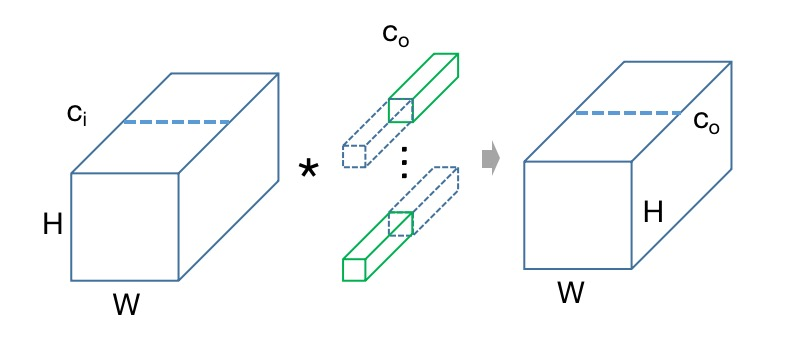
\includegraphics[]{../pic/GC.jpg}}
        \label{fig:Spoon-net}
        \end{minipage}
        }
        \caption[]{组卷积与普通卷积的区别。}
        %英文标题begin
        \addtocounter{figure}{-1}
        \vspace{-5pt}
        %\SetEnglishCaption
        \renewcommand{\figurename}{Fig}
        \caption{The difference between group convolution and ordinary convolution}
        \renewcommand{\figurename}{图}
        %英文标题end
        \label{pic:GC}
\end{figure}

组卷积也是轻量化模型的重要手段。假设输入有$c_i$层特征图,每个特征图都是$H*W$,$3*3$的卷积核$c_o$个,普通卷积将进行$H*W*3*3*c_i*c_o$次乘法计算;若将其分为$g$组,整个卷积过程只会进行$H*W*3*3*(c_i/g)*c_o$次乘法,计算量变为原来的$\frac{1}{g}$。
同样,参数个数也变为原来的$\frac{1}{g}$,减少了模型过拟合的风险。

为了保证稳定性和精度,S-Net的网络设计还包括:

a) 上采样方式选择双线性插值法。
% 上采样的方式一般有三种:反池化,反卷积,插值法。反池化是速度最快的上采样操作,计算量和参数也特别少,但是准确率一般。虽然理论上,反卷积由于具有更多的参数,可以更好的学习特征,Odena等人\upcite{odena2016deconvolution}的研究表明,如果参数学习不当,反卷积很容易出现输出特征图带有明显棋盘状的现象,双线性插值可以取得与反卷积相同甚至更好的效果。因此,我们选择参数少且容易取得较好效果的双线性插值法。

b) 在卷积之后,激活函数之前,加入批归一化层\upcite{ioffe2015batch}加快模型收敛(Batch Normalization,简称BN)。

\begin{equation}
    {BN}(x) = \gamma\frac{x-\mu}{\sigma}+\beta
\end{equation}

c) 激活函数以$ReLU$函数为主。本文中几乎所有的激活函数都是$ReLU$函数,即:
\begin{equation}
    {ReLU}(x)=\left\{
    \begin{aligned}
        x, & &\text{if} & & x > 0 \\
        0, & &\text{if} & & x \leq 0
    \end{aligned}
    \right.
\end{equation}
$ReLU$由于非负区间的梯度为常数,可以缓解梯度消失问题,使得模型的收敛速度维持在一个稳定状态。

在最后一层卷积层,激活函数会使用$Sigmoid$函数,即:${Sigmoid}(x)=\frac{1}{1+e^{-x}}$用于将输出映射到0-1之间,代表该像素点为云的概率。

d) 损失函数采用交叉熵损失函数,用$L$表示,即:
\begin{equation}
    {L} = -\sum_{i=1}^N y_ilog(\hat{y}_i)+(1-y_i)log(1-\hat{y}_i)
\end{equation}
其中,$N$表示所有所有样本个数,$y_i$代表标签真值,$\hat{y_i}$代表模型预测值。
并且我们的损失函数包括两部分,如图\ref{pic:loss}所示,分别计算光谱特征提取与空间特征提取阶段的损失。
\begin{figure}[H]
    \centering
    \resizebox{\linewidth}{!}{
    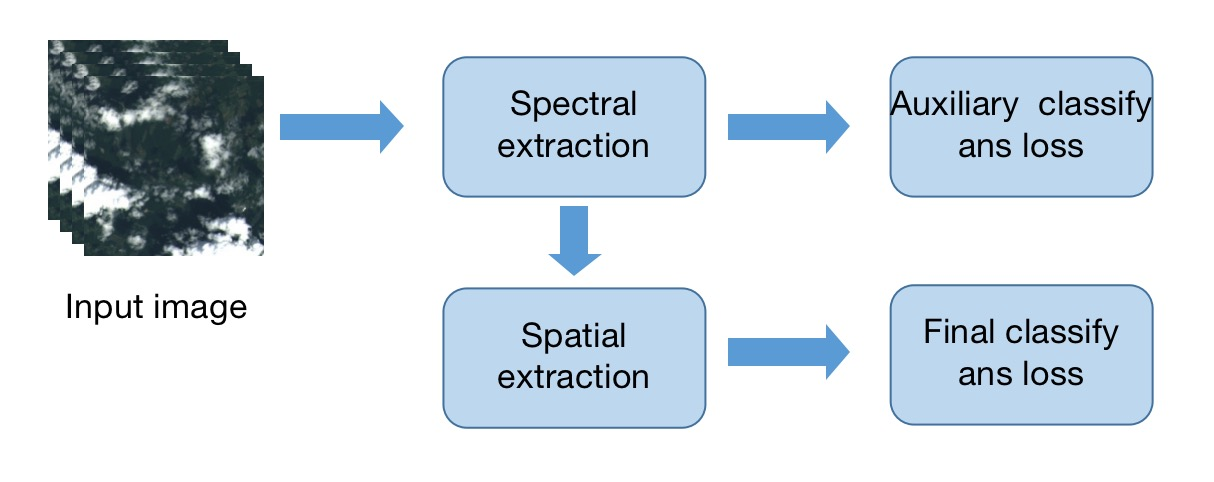
\includegraphics[scale=1]{../pic/loss.jpg}}
    \caption[]{两阶段损失,光谱特征提取阶段与空间特征提取阶段各有一个损失。}
    %英文标题begin
    \addtocounter{figure}{-1}
    \vspace{-5pt}
    %\SetEnglishCaption
    \renewcommand{\figurename}{Fig}
    \caption{Two stages of loss, one each for the spectral feature extraction stage and the spatial feature extraction stage}
    \renewcommand{\figurename}{图}
    %英文标题end
    \label{pic:loss}
\end{figure}

\section[]{实验与分析}

本文将S-Net的分割结果与CFMask(FMask\upcite{zhu2012object}的C语言实现)、U-Net\upcite{ronneberger2015unet}的分割结果做比较。Foga等人\upcite{foga2017cloud_data}使用多种传统方法在Landsat8 biome数据集上进行实验,结果表明FMask是最优秀的方法。同时FMask也是Landsat官方生成质量评估(QA)波段所用的方法。U-Net是图像分割领域中经典的深度学习方法,Jeppesena等人\upcite{jeppesen2019cloud}使用U-Net在Landsat8 biome数据集上进行的实验取得了很好的效果。而且S-Net的空间特征提取部分也借鉴了U-Net的思想。因此,将S-Net的分割结果与CFMask、U-Net的分割结果做比较具有较高的说服力。

输入是除了全色波段的其余10个波段,将所有图像按6:4随机划分为训练集和测试集,并调整U-Net的输入通道数为10。将地物真实标签(Ground Truth,简称GT)分为云与非云两类。Chai等人\upcite{chai2019cloud}的研究表明输入DN值(Digital number)或大气顶部反射率(ToA)数据,会取得相似的结果,我们选择使用DN值作为模型输入,并为了使训练更加稳定,对输入进行归一化。
具体参数,如学习率为$1e^{-2}$,批训练大小为 8,采用动量为0.9的随机梯度下降法训练,动态调整辅助损失与主损失的比例,辅助损失的权重逐渐降低,主损失的权重逐渐增高,权重的变化分为3个阶段:(0.8, 0.2)、(0.2, 0.8)、(0, 1)。
本文所有实验均在深度学习框架Pytorch上进行,操作系统为Ubuntu 16.04,处理器为NVIDIA Titan XP, 内存16 GB。

为客观评定算法的有效性和优越性,采用准确率(Acc),召回率(Rec),精确度(Prec),$\rm F_1$值对结果进行评估。其中,准确率衡量像素分类正确的概率;召回率衡量属于云的像素中被分类正确的概率,是漏警率的相反数;精确度衡量被识别为云的像素中真正是云的概率,是虚警率的相反数;$\rm F_1$值是召回率与精确度的调和平均数,常被用于二分类问题,可以有效衡量样本不均衡时检测结果的好坏。

\subsection{整体评估}
在Landsat8 Biome数据集上的实验结果如表(\ref{tab_eval})所示,一共包括8种下垫面(即:裸土、森林、草地/农田、灌木、冰雪、城市、水、湿地)。
结果表明,S-Net在几乎所有下垫面上的检测结果均优于U-Net和CFmask(除了城市稍落后于U-Net)。S-Net的检测结果有0.9505的平均$\rm F_1$值,高于U-Net的0.9352和CFMask的0.86;也有95.34\%的平均准确率(Acc),高于U-Net的94.15\%和CFMask的86.09\%。虽然平均精确度(Prec)略低于U-Net(0.3\%),但平均召回率(Rec)达到了95.15\%,比U-Net高3.15\%。需要强调的是,我们的模型非常轻量,参数量只有0.34M个,是U-Net(28M个)的八十分之一。

\end{multicols}

\begin{table}[H]
    \caption{在Landsat8 Biome数据集上,S-Net、U-Net、CFMask实验结果对比}
    %英文标题begin
    \addtocounter{table}{-1}
    \vspace{-5pt}
    %\SetEnglishCaption
    \renewcommand{\figurename}{Tab}
    \caption{Comparison of S-Net, U-Net, CFMask experimental results on Landsat8 Biome dataset}
    \vspace{5pt}
    \renewcommand{\figurename}{表}
    %英文标题end
    \centering
    \resizebox{0.9\textwidth}{!}{
    \begin{tabular}{c|cccccccccc}
        \hline
        模型 & 指标& 裸土& 森林& 草地/农田& 灌木& 冰雪& 城市& 水&  湿地& 所有下垫面\\
        \hline
        \multirow{4}*{S-Net}
        &Acc   &96.43 &96.61 &94.48 &95.08 &96.29 &94.85 &94.38 &94.56 &\textbf{95.34}\\
        &Rec.  &96.46 &95.90 &92.67 &93.21 &95.38 &97.07 &91.90 &98.60 &\textbf{95.15}\\
        &Prec. &97.89 &99.38 &93.10 &97.41 &95.61 &91.57 &92.82 &92.34 &95.01\\
        &$\rm F_1$    &97.17 &97.61 &92.89 &95.26 &95.50 &94.24 &92.36 &95.37 &\textbf{95.05}\\
        \hline
        \multirow{4}*{U-Net}
        &Acc   &96.09 &94.51 &92.67 &94.48 &91.78 &95.00 &93.74 &94.90 &94.15\\
        &Rec.  &96.00 &92.96 &81.91 &91.58 &89.16 &96.22 &89.83 &98.34 &92.00\\
        &Prec. &97.60 &99.22 &97.31 &97.77 &90.90 &92.56 &93.97 &93.05 &\textbf{95.30}\\
        &$\rm F_1$    &96.80 &95.99 &88.95 &94.58 &90.02 &94.36 &91.85 &95.62 &93.52\\
        \hline
        \multirow{4}*{CFMask}
        &Acc   &87.46 &95.20 &85.42 &90.34 &60.97 &83.05 &91.51 &90.78 &86.09\\
        &Rec.  &90.85 &93.87 &68.03 &92.04 &92.21 &96.07 &92.22 &96.37 &91.45\\
        &Prec. &88.99 &99.31 &88.85 &89.83 &51.74 &73.25 &86.97 &88.38 &82.89\\
        &$\rm F_1$     &89.91 &96.51 &77.05 &90.92 &66.29 &83.13 &89.52 &92.21 &86.96\\
        \hline
    \end{tabular}}
    
    \label{tab_eval}
\end{table}

\begin{multicols}{2}

同时可以发现,我们的模型对于碎云、细节有良好的检测与保持能力。U-Net的识别更加光滑,使得一些细节被忽略,而我们的模型更加注重细节,这对于云检测是一个很重要的能力。如图\ref{Fig.main1}所示,从左到右依次为真彩色图、人工标注、光谱特征提取结果构成的假彩色图、我们的模型预测结果、U-Net结果,白色代表云,黑色代表非云,偶数行的图像是奇数行图像中黄色方框部分的放大结果,黄色方框的大小为$20*20$。

\end{multicols}

\begin{figure}[H]
    \centering
    \resizebox{0.9\linewidth}{!}{
    \subfigure[真彩色图]{
        \begin{minipage}[b]{0.15\linewidth}
            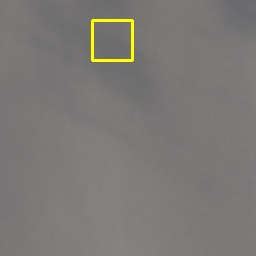
\includegraphics[width=1\linewidth]{../log/spoon2/cut/LC81321192014054LGN00_03055_color.jpg}\vspace{4pt}
            
\includegraphics[width=1\linewidth]{../log/spoon2/cut/tmp_cut_LC81321192014054LGN00_03055_color.jpg}\vspace{4pt}
            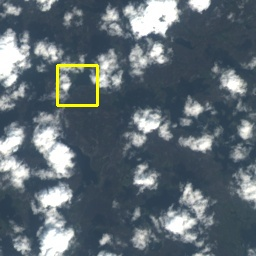
\includegraphics[width=1\linewidth]{../log/spoon2/cut/LC80350192014190LGN00_06561_color.jpg}\vspace{4pt}
            
\includegraphics[width=1\linewidth]{../log/spoon2/cut/tmp_cut_LC80350192014190LGN00_06561_color.jpg}\vspace{4pt}
            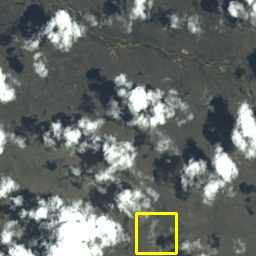
\includegraphics[width=1\linewidth]{../log/spoon2/cut/LC80980712014024LGN00_15443_color.jpg}\vspace{4pt}
            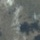
\includegraphics[width=1\linewidth]{../log/spoon2/cut/tmp_cut_LC80980712014024LGN00_15443_color.jpg}\vspace{4pt}
        \end{minipage}
    }
    \subfigure[人工标签]{
        \begin{minipage}[b]{0.15\linewidth}
            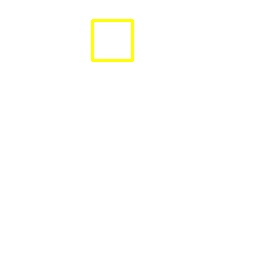
\includegraphics[width=1\linewidth]{../log/spoon2/cut/LC81321192014054LGN00_03055_mask.jpg}\vspace{4pt}
            
\includegraphics[width=1\linewidth]{../log/spoon2/cut/tmp_cut_LC81321192014054LGN00_03055_mask.jpg}\vspace{4pt}
            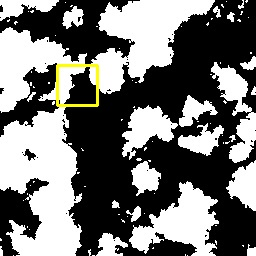
\includegraphics[width=1\linewidth]{../log/spoon2/cut/LC80350192014190LGN00_06561_mask.jpg}\vspace{4pt}
            
\includegraphics[width=1\linewidth]{../log/spoon2/cut/tmp_cut_LC80350192014190LGN00_06561_mask.jpg}\vspace{4pt}
            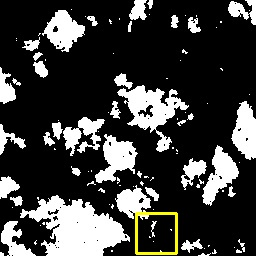
\includegraphics[width=1\linewidth]{../log/spoon2/cut/LC80980712014024LGN00_15443_mask.jpg}\vspace{4pt}
            
\includegraphics[width=1\linewidth]{../log/spoon2/cut/tmp_cut_LC80980712014024LGN00_15443_mask.jpg}\vspace{4pt}
        \end{minipage}
    }
    \subfigure[光谱特征]{
        \begin{minipage}[b]{0.15\linewidth}
            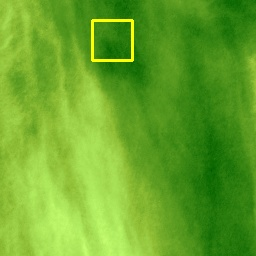
\includegraphics[width=1\linewidth]{../log/spoon2/cut/LC81321192014054LGN00_03055_spectral.jpg}\vspace{4pt}
            
\includegraphics[width=1\linewidth]{../log/spoon2/cut/tmp_cut_LC81321192014054LGN00_03055_spectral.jpg}\vspace{4pt}
            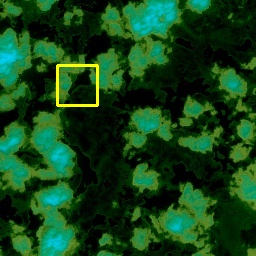
\includegraphics[width=1\linewidth]{../log/spoon2/cut/LC80350192014190LGN00_06561_spectral.jpg}\vspace{4pt}
            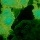
\includegraphics[width=1\linewidth]{../log/spoon2/cut/tmp_cut_LC80350192014190LGN00_06561_spectral.jpg}\vspace{4pt}
            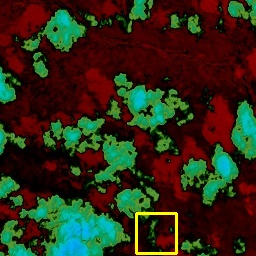
\includegraphics[width=1\linewidth]{../log/spoon2/cut/LC80980712014024LGN00_15443_spectral.jpg}\vspace{4pt}
            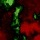
\includegraphics[width=1\linewidth]{../log/spoon2/cut/tmp_cut_LC80980712014024LGN00_15443_spectral.jpg}\vspace{4pt}
        \end{minipage}
    }
    \subfigure[S-Net]{
        \begin{minipage}[b]{0.15\linewidth}
            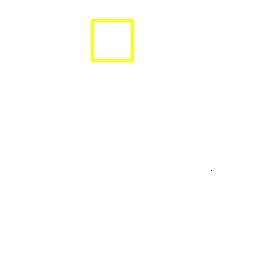
\includegraphics[width=1\linewidth]{../log/spoon2/cut/LC81321192014054LGN00_03055_my.jpg}\vspace{4pt}
            
\includegraphics[width=1\linewidth]{../log/spoon2/cut/tmp_cut_LC81321192014054LGN00_03055_my.jpg}\vspace{4pt}
            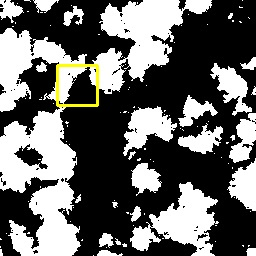
\includegraphics[width=1\linewidth]{../log/spoon2/cut/LC80350192014190LGN00_06561_my.jpg}\vspace{4pt}
            
\includegraphics[width=1\linewidth]{../log/spoon2/cut/tmp_cut_LC80350192014190LGN00_06561_my.jpg}\vspace{4pt}
            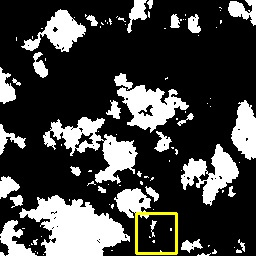
\includegraphics[width=1\linewidth]{../log/spoon2/cut/LC80980712014024LGN00_15443_my.jpg}\vspace{4pt}
            
\includegraphics[width=1\linewidth]{../log/spoon2/cut/tmp_cut_LC80980712014024LGN00_15443_my.jpg}\vspace{4pt}
        \end{minipage}
    }
    \subfigure[U-Net]{
        \begin{minipage}[b]{0.15\linewidth}
            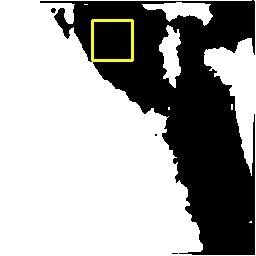
\includegraphics[width=1\linewidth]{../log/spoon2/cut/LC81321192014054LGN00_03055_unet.jpg}\vspace{4pt}
            
\includegraphics[width=1\linewidth]{../log/spoon2/cut/tmp_cut_LC81321192014054LGN00_03055_unet.jpg}\vspace{4pt}
            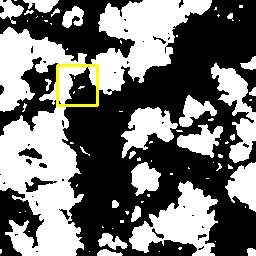
\includegraphics[width=1\linewidth]{../log/spoon2/cut/LC80350192014190LGN00_06561_unet.jpg}\vspace{4pt}
            
\includegraphics[width=1\linewidth]{../log/spoon2/cut/tmp_cut_LC80350192014190LGN00_06561_unet.jpg}\vspace{4pt}
            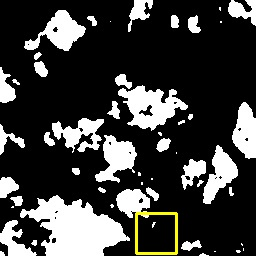
\includegraphics[width=1\linewidth]{../log/spoon2/cut/LC80980712014024LGN00_15443_unet.jpg}\vspace{4pt}
            
\includegraphics[width=1\linewidth]{../log/spoon2/cut/tmp_cut_LC80980712014024LGN00_15443_unet.jpg}\vspace{4pt}
        \end{minipage}
    }
    }
\caption{Spoon-Net检测结果展示,偶数行是奇数行黄色方框部分的放大图。}
%英文标题begin
\addtocounter{figure}{-1}
\vspace{-5pt}
%\SetEnglishCaption
\renewcommand{\figurename}{Fig}
\caption{Example of spoon-net results, even lines are enlarged views of the yellow boxes of odd lines}
\renewcommand{\figurename}{图}
%英文标题end
\label{Fig.main1}
\end{figure}

\begin{multicols}{2}

% 我们对第一阶段输出的光谱特征个数进行实验。实验发现,当光谱特征数为3时,具有最高的分类精度与f1值。

% \begin{table}[H]
%     \caption{光谱特征提取层数对实验结果的影响}
%     %英文标题begin
%     \addtocounter{table}{-1}
%     \vspace{-5pt}
%     %\SetEnglishCaption
%     \renewcommand{\tablename}{Tab}
%     \caption{Influence of the number of spectral feature extraction layers on experimental results}
%     \renewcommand{\tablename}{表}
%     \vspace{5pt}
%     %英文标题end

%     \centering
%     \resizebox{\linewidth}{!}{
%     \begin{tabular}{cccc}
%     \hline
%     光谱层数& acc& f1& 参数数量\\
%     \hline
%     2&	94.38&  94.11& 238K\\
%     3&  \textbf{95.34}&  \textbf{95.05}& 342K\\
%     4&  94.79&  94.46& 450K\\
%     5&  94.92&  94.60& 562K\\
%     6&  94.84&  94.61& 678K\\
%     \hline
%     \end{tabular}}
    
%     \label{BiomeFlag}
%     \end{table}

% 我们减少encoder-decoder层数(一般会是4层)。由于光谱特征提取部分的存在,在这一部分模型提取空间信息的压力已经被大大减小,所以我们并不需要很深的网络、很多的参数去拟合很复杂的空间特征,而随着层数的减少,参数量几乎是几何减少的。实验发现,当encoder-decoder层数大于2时,云检测效果不会再有提高。

% \begin{table}[H]
%     \caption{光谱特征提取层数对实验结果的影响}
%     %英文标题begin
%     \addtocounter{table}{-1}
%     \vspace{-5pt}
%     %\SetEnglishCaption
%     \renewcommand{\tablename}{Tab}
%     \caption{Influence of the number of spectral feature extraction layers on experimental results}
%     \renewcommand{\tablename}{表}
%     \vspace{5pt}
%     %英文标题end

%     \centering
%     \resizebox{0.9\linewidth}{14mm}{
%     \begin{tabular}{cccc}
%     \hline
%     下采样层数& acc& f1& 参数数量\\
%     \hline
%     1&	92.33&  92.12& 72K\\
%     2&  \textbf{95.34}&  \textbf{95.05}& 341K\\
%     3&  95.01&  94.89& 1.4M\\
%     4&  94.87&  94.62& 5.7M\\
%     \hline
%     \end{tabular}}
    
%     \label{BiomeFlag}
%     \end{table}

% \subsection{轻量化}
% 我们的模型参数量有0.34M个,而U-Net的模型参数有28M个。S-Net如此轻量主要有三方面原因:
% \begin{enumerate}[1.]
%     \item 使用$1*1$的卷积核进行图像的光谱特征提取。$1*1$的卷积核是相同个数的$3*3$卷积核的九分之一。
%     \item 使用浅层的encoder-decoder框架提取空间特征。U-Net网络参数多的主要原因是具有更深的encoder-decoder结构,以U-Net为例,U-Net最深一层就有14M的参数,占据了所有参数的一半。由于拥有光谱特征提取阶段,S-Net可以不需要很大的感受野,从而节省大量参数。
%     \item 使用组卷积代替普通卷积。假设将卷积核分为$g$组,组卷积的参数个数是普通卷积的$\frac{1}{g}$.
% \end{enumerate}

\subsection{碎云检测评估}
为衡量模型对碎云的检测能力,我们定义碎云为:面积(四连通)小于30个像素的云。由于此时计算准确率(Acc)已无意义,所我们选择召回率(Rec)、精确度(Prec)和$\rm F_1$值作为衡量准则。实验表明,在识别碎云时,S-Net拥有0.1818的平均$\rm F_1$值,显著高于U-Net的0.118,并且在除了森林外的所有下垫面上均优于U-Net。

\end{multicols}
\begin{table}[H]
    \caption{在Landsat8 Biome数据集上,S-Net、U-Net、CFMask对碎云的检测结果对比}
    %英文标题begin
    \addtocounter{table}{-1}
    \vspace{-5pt}
    %\SetEnglishCaption
    \renewcommand{\figurename}{Tab}
    \caption{On the Landsat8 Biome data set, S-Net, U-Net, CFMask compare the detection results of broken clouds}
    \vspace{5pt}
    \renewcommand{\figurename}{表}
    %英文标题end
    \centering
    \resizebox{0.9\textwidth}{!}{
    \begin{tabular}{c|cccccccccc}
        \hline
        模型 & 指标& 裸土& 森林& 草地/农田& 灌木& 冰雪& 城市& 水&  湿地& 所有下垫面\\
        \hline
        \multirow{4}*{S-Net}
        &Rec.  &7.82 &23.14 &21.84 &15.28 &8.78 &21.22 &17.61 &17.65 &\textbf{16.67}\\
        &Prec. &14.79 &28.08 &24.42 &22.27 &9.06 &15.28 &19.93 &34.15 &\textbf{21.00}\\
        &$\rm F_1$     &10.23 &25.37 &23.06 &18.13 &8.92 &17.77 &18.70 &23.27 &\textbf{18.18}\\
        \hline
        \multirow{4}*{U-Net}
        &Rec.  &5.98 &6.63 &13.12 &10.00 &2.66 &13.43 &6.45 &13.84 &9.01\\
        &Prec. &16.64 &14.24 &28.86 &20.49 &2.88 &16.81 &11.28 &31.17 &17.79\\
        &$\rm F_1$     &8.80 &9.05 &18.04 &13.44 &2.77 &14.93 &8.21 &19.17 &11.80\\
        \hline
        \multirow{4}*{CFMask}
        &Rec.  &5.14 &48.82 &15.32 &18.20 &3.45 &16.98 &20.18 &13.54 &17.70\\
        &Prec. &1.66 &32.98 &7.50 &5.96 &0.25 &5.95 &3.56 &5.69 &7.94\\
        &$\rm F_1$     &2.51 &39.37 &10.07 &8.98 &0.47 &8.81 &6.05 &8.01 &10.53\\
        \hline
    \end{tabular}}
    
    \label{tab_eval_2}
\end{table}

\begin{multicols}{2}

虽然在检测碎云时,S-Net的表现显著优于U-Net,但$\rm F_1$也仍不到0.2。原因可能有两点:1. 检测碎云具有较高的难度;2. 人工在标注碎云时存在困难,数据存在错误。Scaramuzza等人\upcite{scaramuzza2011development}的研究表明人工标注的数据可能存在7\%左右的错误。尤其对于碎云,人工标注更加不准确,且碎云数量较小,对错误标签更加敏感。我们发现,'L8 Biome'数据确实存在一些问题,图\ref{Fig.main2}展示了一些存在问题的图像样本。同时,由于人工标注的不稳定性,简单地依靠评价指标可能并不能真实反应模型的优劣,因为大部分模型都很容易对于大面积的厚云(低下垫面信息的)有较好的识别能力;并且以这些标签为真值进行的训练,可能也会存在问题。

\begin{figure}[H]
    \centering
    \subfigure[真彩色图]{
        \begin{minipage}[b]{0.15\linewidth}
            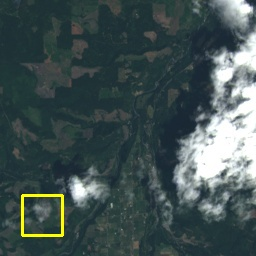
\includegraphics[width=1\linewidth]{../log/spoon2/cut2/LC80460282014171LGN00_12434_color.jpg}\vspace{4pt}
            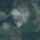
\includegraphics[width=1\linewidth]{../log/spoon2/cut2/tmp_cut_LC80460282014171LGN00_12434_color.jpg}\vspace{4pt}
            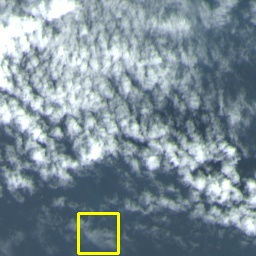
\includegraphics[width=1\linewidth]{../log/spoon2/cut2/LC81620432014072LGN00_16237_color.jpg}\vspace{4pt}
            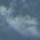
\includegraphics[width=1\linewidth]{../log/spoon2/cut2/tmp_cut_LC81620432014072LGN00_16237_color.jpg}\vspace{4pt}
            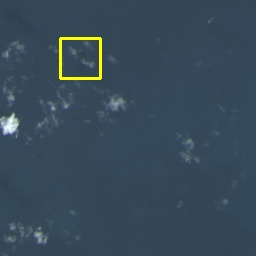
\includegraphics[width=1\linewidth]{../log/spoon2/cut2/LC81620432014072LGN00_16329_color.jpg}\vspace{4pt}
            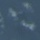
\includegraphics[width=1\linewidth]{../log/spoon2/cut2/tmp_cut_LC81620432014072LGN00_16329_color.jpg}\vspace{4pt}
        \end{minipage}
    }
    \subfigure[人工标签]{
        \begin{minipage}[b]{0.15\linewidth}
            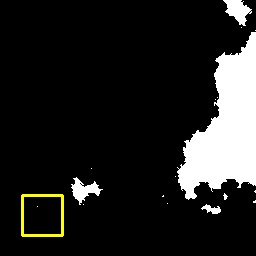
\includegraphics[width=1\linewidth]{../log/spoon2/cut2/LC80460282014171LGN00_12434_mask.jpg}\vspace{4pt}
            
\includegraphics[width=1\linewidth]{../log/spoon2/cut2/tmp_cut_LC80460282014171LGN00_12434_mask.jpg}\vspace{4pt}
            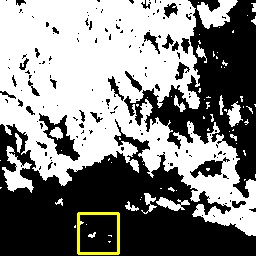
\includegraphics[width=1\linewidth]{../log/spoon2/cut2/LC81620432014072LGN00_16237_mask.jpg}\vspace{4pt}
            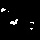
\includegraphics[width=1\linewidth]{../log/spoon2/cut2/tmp_cut_LC81620432014072LGN00_16237_mask.jpg}\vspace{4pt}
            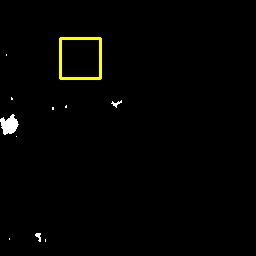
\includegraphics[width=1\linewidth]{../log/spoon2/cut2/LC81620432014072LGN00_16329_mask.jpg}\vspace{4pt}
            \includegraphics[width=1\linewidth]{../log/spoon2/cut2/tmp_cut_LC81620432014072LGN00_16329_mask.jpg}\vspace{4pt}
        \end{minipage}
    }
    \subfigure[光谱特征]{
        \begin{minipage}[b]{0.15\linewidth}
            \includegraphics[width=1\linewidth]{../log/spoon2/cut2/LC80460282014171LGN00_12434_spectral.jpg}\vspace{4pt}
            \includegraphics[width=1\linewidth]{../log/spoon2/cut2/tmp_cut_LC80460282014171LGN00_12434_spectral.jpg}\vspace{4pt}
            \includegraphics[width=1\linewidth]{../log/spoon2/cut2/LC81620432014072LGN00_16237_spectral.jpg}\vspace{4pt}
            \includegraphics[width=1\linewidth]{../log/spoon2/cut2/tmp_cut_LC81620432014072LGN00_16237_spectral.jpg}\vspace{4pt}
            \includegraphics[width=1\linewidth]{../log/spoon2/cut2/LC81620432014072LGN00_16329_spectral.jpg}\vspace{4pt}
            \includegraphics[width=1\linewidth]{../log/spoon2/cut2/tmp_cut_LC81620432014072LGN00_16329_spectral.jpg}\vspace{4pt}
        \end{minipage}
    }
    \subfigure[S-Net]{
        \begin{minipage}[b]{0.15\linewidth}
            \includegraphics[width=1\linewidth]{../log/spoon2/cut2/LC80460282014171LGN00_12434_my.jpg}\vspace{4pt}
            \includegraphics[width=1\linewidth]{../log/spoon2/cut2/tmp_cut_LC80460282014171LGN00_12434_my.jpg}\vspace{4pt}
            \includegraphics[width=1\linewidth]{../log/spoon2/cut2/LC81620432014072LGN00_16237_my.jpg}\vspace{4pt}
            \includegraphics[width=1\linewidth]{../log/spoon2/cut2/tmp_cut_LC81620432014072LGN00_16237_my.jpg}\vspace{4pt}
            \includegraphics[width=1\linewidth]{../log/spoon2/cut2/LC81620432014072LGN00_16329_my.jpg}\vspace{4pt}
            \includegraphics[width=1\linewidth]{../log/spoon2/cut2/tmp_cut_LC81620432014072LGN00_16329_my.jpg}\vspace{4pt}
        \end{minipage}
    }
    \subfigure[U-Net]{
        \begin{minipage}[b]{0.15\linewidth}
            \includegraphics[width=1\linewidth]{../log/spoon2/cut2/LC80460282014171LGN00_12434_unet.jpg}\vspace{4pt}
            \includegraphics[width=1\linewidth]{../log/spoon2/cut2/tmp_cut_LC80460282014171LGN00_12434_unet.jpg}\vspace{4pt}
            \includegraphics[width=1\linewidth]{../log/spoon2/cut2/LC81620432014072LGN00_16237_unet.jpg}\vspace{4pt}
            \includegraphics[width=1\linewidth]{../log/spoon2/cut2/tmp_cut_LC81620432014072LGN00_16237_unet.jpg}\vspace{4pt}
            \includegraphics[width=1\linewidth]{../log/spoon2/cut2/LC81620432014072LGN00_16329_unet.jpg}\vspace{4pt}
            \includegraphics[width=1\linewidth]{../log/spoon2/cut2/tmp_cut_LC81620432014072LGN00_16329_unet.jpg}\vspace{4pt}
        \end{minipage}
    }
\caption{问题标签}
%英文标题begin
\addtocounter{figure}{-1}
\vspace{-5pt}
%\SetEnglishCaption
\renewcommand{\figurename}{Fig}
\caption{Error label}
\renewcommand{\figurename}{图}
%英文标题end
\label{Fig.main2}
\end{figure}

\section[]{结论}
云检测一直是遥感领域的研究热点与难点。本文提出了一种两阶段的遥感图像云检测模型。相比于现有的深度学习模型,我们的模型更加轻量,并且具有更好的保持边缘细节的能力和对小的碎云的检测能力。我们注重遥感图像光谱特征的提取,在第一阶段利用$1*1$的卷积核专门提取光谱特征,使得检测结果保持了“纯粹性”,没有受到其空间信息的干扰,并使其直达最终的分类层。再利用浅层encoder-decoder结构,引入组卷积,对每个光谱特征分别计算空间信息。该模型充分利用遥感图像多波段的特点,有效解决了现有方法在保持边缘细节与扩大感受野之间的矛盾,并在Landsat8数据集上达到了95.34\%的准确率,基本还原了输入影像的细节信息。后续将继续优化光谱特征与空间特征提取部分,并尝试深度学习与传统方法结合,以实现更加精确的遥感图像云检测。

\bibliography{./ref.bib}
\end{multicols}
\end{document}
